\documentclass{article}
\usepackage[table]{xcolor}
\usepackage{array}
\usepackage{booktabs}
\usepackage{colortbl}
\usepackage{geometry}
\usepackage{tikz}
\usetikzlibrary{shapes,arrows,positioning}

% Set minimal margins
\geometry{a4paper, left=1cm, right=1cm, top=2cm, bottom=1cm}

% Color definitions
\definecolor{headerbg}{RGB}{44,62,80}
\definecolor{row1}{RGB}{236,240,241}
\definecolor{row2}{RGB}{255,255,255}
\definecolor{commandbg}{RGB}{52,152,219}

\begin{document}

\centering
{\Large \bfseries \color{headerbg} Web Application Reconnaissance}

\vspace{0.5cm}

\renewcommand{\arraystretch}{2}
\begin{tabular}{>{\ttfamily}p{0.45\textwidth} >{\raggedright\arraybackslash}p{0.50\textwidth}}
\toprule
\rowcolor{headerbg}
\color{white}\textbf{Command} & \color{white}\textbf{Description} \\
\midrule
\rowcolor{row1}
\textcolor{commandbg}{subfinder -d target.com > subf.txt} & 
Discovers subdomains using passive sources and saves to file \\
\rowcolor{row2}
\textcolor{commandbg}{assetfinder -subs-only target.com > ast.txt} & 
Finds domains and subdomains related to target and saves to file \\
\rowcolor{row1}
\textcolor{commandbg}{cat subf.txt ast.txt | sort -u | tee subdomains.txt} & 
Combines and deduplicates subdomain lists \\
\rowcolor{row2}
\textcolor{commandbg}{cat subdomains.txt | httpx | tee liveSubdomains.txt} & 
Probes for live subdomains (HTTP servers) \\
\rowcolor{row1}
\textcolor{commandbg}{cat liveSubdomains.txt | gau | tee gau.txt} & 
Fetches historical URLs from AlienVault OTX \\
\rowcolor{row2}
\textcolor{commandbg}{cat liveSubdomains.txt | waybackurls | tee wayback.txt} & 
Extracts URLs from Wayback Machine archives \\
\rowcolor{row1}
\textcolor{commandbg}{cat gau.txt wayback.txt | sort -u | tee urls.txt} & 
Merges and deduplicates all discovered URLs \\
\rowcolor{row2}
\textcolor{commandbg}{cat urls.txt | fff | tee liveUrls.txt} & 
Fetches URLs and saves responses with metadata \\

\bottomrule
\end{tabular}

\vspace*{2cm}

\begin{center}
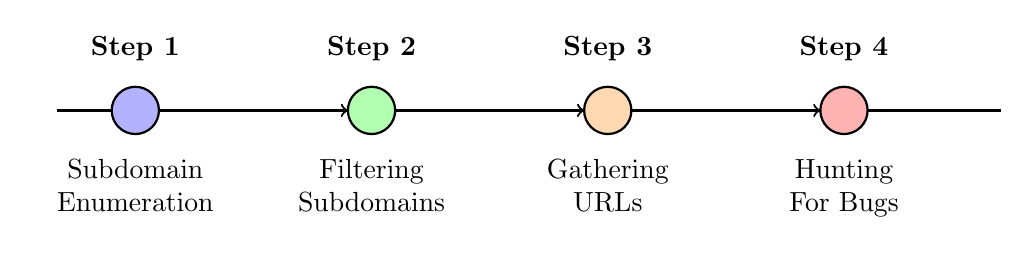
\begin{tikzpicture}
% Timeline
\draw[thick] (0,0) -- (12,0);

% Steps
\foreach \x/\step/\color in {1/Subdomain Enumeration/blue, 4/Filtering Subdomains/green, 7/Gathering URLs/orange, 10/Hunting For Bugs/red} {
    \draw[thick, fill=\color!30] (\x,0) circle (0.3);
    \node[above] at (\x,0.5) {\textbf{Step \the\numexpr\x/3+1}};
    \node[below, text width=2.5cm, align=center] at (\x,-0.5) {\step};
}

% Arrows
\draw[->, thick] (1.3,0) -- (3.7,0);
\draw[->, thick] (4.3,0) -- (6.7,0);
\draw[->, thick] (7.3,0) -- (9.7,0);

\end{tikzpicture}
\end{center}

\end{document}